\documentclass{scrreport}
\usepackage[utf8]{inputenc}
\usepackage{float} 
\usepackage{graphicx}
\usepackage{hyperref}

% Add any additional packages you may need here

\renewcommand*{\thesection}{\Roman{section}}
\renewcommand*{\thesubsection}{\arabic{subsection}}
\renewcommand*{\thesubsubsection}{\roman{subsubsection}}

\title{Security Oracles - a new active approach to Smart Contracts Security}
\subtitle{Milestone Report}

\author{Team Sentinel}
\date{11/04/2024}

\graphicspath{Images/}

\begin{document}

\maketitle

\tableofcontents


\chapter{Cardano Smart Contract Security}
\label{chap:introduction}

\section{State of Affairs}

As of April 2024, the Cardano smart contract ecosystem is perceived as highly resilient \
to attacks and exploits, positioning itself as a significant entity in the landscape of \
blockchain security. This perceived robustness is largely attributed to the collaborative \ 
efforts of its foundational bodies and ecosystem contributors, notably Input Output Global (IOG) \
and the Cardano Foundation.

A key factor contributing to Cardano's security strength is the formal and precise nature of its \
smart contract languages. In addition, unlike account-based blockchains such as Ethereum, where \
the code is human-readable, Cardano employs Plutus Core in binary form. This design not only makes \
it challenging for adversaries to scrutinize the code directly but also reflects the platform's \
commitment to a mathematically rigorous foundation for smart contracts. This architecture decisively \
minimizes the opportunities for exploits.

The security acclaim of Cardano also stems from its development philosophy, which is heavily anchored \
in academic rigor and peer-reviewed research, courtesy of IOG and the Cardano Foundation. This methodical \
approach contrasts sharply with the more experimental strategies seen on other platforms and has been \
integral to its security success.

Community engagement and proactive security measures have further solidified Cardano's standing. \
With notable auditing entities like Runtime Verification and Tweag leading the charge, bolstered \
by initiatives such as CIP 68 for audit standards, Cardano established a preemptively secure environment \
for its dApps ecosystem. These efforts, along with enticing bug bounties from various DeFi platforms, have \
been pivotal in maintaining an attractive yet secure platform for developers and users alike.

The establishment of the Certification Working Group by IOG marked a significant stride in institutionalizing \
security practices. The group's efforts culminated in the creation of several critical CIPs, including CIP 68 \
for audit standards, CIP 72 for dApp registration, and CIP 96 for on-chain dApp certification. These measures \
provide an added security assurance layer for user interactions within the Cardano ecosystem. The Working Group's \
evolution into Intersec, aimed at advancing these initiatives in the Voltaire Era, underscores the sustained \
commitment to security excellence.

Moreover, the Certification Group's proactive approach in cataloging vulnerabilities and promoting standardized \
reporting methodologies has been embraced by leading security firms auditing Cardano dApps. This collective \
vigilance and structured approach to security underscore Cardano's robust defensive posture in the dynamic \
landscape of blockchain technology.

It is important to note, however, that smart contract support on Cardano was introduced later compared to other \
platforms. As a consequence, the Cardano DeFi ecosystem was not initially seen as an attractive target by attackers, \
largely due to its nascent stage and smaller size relative to the more established ecosystems. This delay \
inadvertently provided a form of security through obscurity, as the ecosystem did not bear the brunt of the \
aggressive hacking attempts that were prevalent during the early development phases of DeFi on other blockchains. \
While this allowed Cardano's DeFi sector to develop without the immediate pressure of high-profile exploits, \
it also meant that its security systems were not tested under the same intense conditions as those of its \
competitors.

\section{Key Vulnerabilities}
Although fairly robust and secure, the Cardano blockchain is not immune to smart contract \
vulnerabilities. This section outlines some key vulnerabilities identified within the Cardano \
ecosystem, highlighting their potential impact. Code audits are the main method through which \
the ecosystem attempts to reduce the impact of these vulnerabilities and develop appropriate \
mitigation strategies.

\begin{enumerate}
    \item \textbf{Datum Hijacking:} Within the Cardano blockchain, each UTxO (Unspent Transaction \
    Output) is associated with a piece of data, known as a Datum, in its Extended UTxO model. \
    This design is intended to enable complex transactions and smart contract interactions. \
    However, a common oversight by some developers is the mistaken assumption that the type of the \
    Datum alone is sufficient to validate the authenticity and intention of a transaction. The \
    reality is that Validators—Cardano smart contracts—must diligently check not just the Datum \
    but also the address associated with the UTxO engaging in the transaction.\

    Neglecting proper address verification can lead to what is known as Datum Hijacking, where \
    malicious entities can exploit a script with a matching Datum type to intercept and redirect \
    outputs that were intended for a different address. This can result in unauthorized actors \
    gaining control over assets, effectively bypassing the security mechanisms that Validators are \
    supposed to enforce.\

    To mitigate this risk, Validators must implement robust verification protocols that confirm \
    the legitimacy of both the Datum and the associated address. This dual-layer check ensures that \
    outputs cannot be hijacked, preserving the integrity of asset control within the smart contract \
    ecosystem.

    \href{https://github.com/input-output-hk/Certification-working-group/blob/vuln-from-audits/Cardano%20Threat%20Intelligence/Vulnerabilities/CTI-2023-ADA-11-01.md}{Additional information}
    
    \item \textbf{Sidechannel Token Name:} In the innovative landscape of Cardano's smart contracts, \
    the minting of tokens is governed by specific policies that ensure the creation process adheres \
    to predefined rules. However, a subtle yet potentially severe vulnerability arises when these \
    minting policies overlook the possibility of including additional tokens with names different \
    from those expected. This oversight paves the way for malicious actors to introduce unauthorized \
    tokens into the ecosystem under the same minting policy, thus posing a significant threat to the \
    integrity and functionality of smart contracts.\

    The essence of this vulnerability lies in the assumption that only tokens with expected names will \
    be minted, disregarding the potential for adversaries to mint additional tokens with different \
    names but within the same policy. Such an action can disrupt the smart contract's intended \
    operations, leading to unauthorized token distribution and potentially compromising the contract's \
    security and reliability.\

    Mitigating this vulnerability requires the implementation of more comprehensive checks within \
    minting policies. Specifically, these policies must not only verify the names of the tokens being \
    minted but also ensure that no extraneous tokens are created during the minting process. By \
    adopting a more rigorous validation approach, smart contracts can prevent the exploitation of \
    this vulnerability, thereby safeguarding the ecosystem against unauthorized token creation and \
    maintaining the sanctity of token distribution protocols.\

    \href{https://github.com/input-output-hk/Certification-working-group/blob/vuln-from-audits/Cardano%20Threat%20Intelligence/Vulnerabilities/CTI-2023-ADA-11-02.md}{Additional information}

    \item \textbf{Stealing Validity Tokens:} The Cardano blockchain architecture allows for the \
    deployment of sophisticated smart contracts, which can leverage validity tokens as a means to \
    confirm transaction authenticity and state. A critical vulnerability emerges when these smart \
    contracts fail to adequately verify the destination addresses for validity tokens. This oversight \
    enables attackers to divert these tokens to unauthorized addresses, thereby undermining the \
    security mechanisms intended to validate transactions and contract states.\

    The core of this vulnerability is the insufficient validation of destination addresses for \
    validity tokens, which are crucial for the proper functioning of smart contracts. Attackers can \
    exploit this gap by redirecting validity tokens to addresses they control, effectively compromising \
    the smart contract's ability to verify its own state or the authenticity of transactions.\

    To mitigate this risk, it is imperative that smart contracts include stringent validation checks \
    for the destination addresses of validity tokens. Ensuring that these tokens are only sent to \
    authorized addresses is vital for maintaining the security and integrity of smart contract \
    operations on the Cardano blockchain. This approach not only prevents unauthorized access and \
    control over these tokens but also reinforces the trust and reliability inherent in the system's \
    transaction verification process.\

    \href{https://github.com/input-output-hk/Certification-working-group/blob/vuln-from-audits/Cardano%20Threat%20Intelligence/Vulnerabilities/CTI-2023-ADA-11-03.md}{Additional information} 

    \item \textbf{Multiple Satisfaction (Double Spending):} A unique aspect of Cardano's blockchain \
    is its ability to execute complex smart contracts, which necessitates a robust mechanism for \
    handling transaction outputs (UTxOs). A notable vulnerability arises in the form of Multiple \
    Satisfaction, where a single UTxO can be erroneously promised to multiple contracts or \
    transactions. This situation typically occurs in naive implementations that fail to properly \
    isolate or track the usage of UTxOs, allowing an attacker to exploit these oversights for \
    double spending.\

    At the heart of this vulnerability is the mishandling of UTxOs, which are fundamental to \
    Cardano's transaction logic. By exploiting this, an attacker can induce a state where a \
    smart contract believes it has exclusive rights to a UTxO, whereas, in reality, the same \
    UTxO has been allocated or spent elsewhere. This can lead to funds being stolen or the \
    integrity of contract transactions being compromised.\

    Mitigation of this vulnerability requires a meticulous approach to contract design and \
    transaction handling. Smart contracts must be engineered to strictly monitor and validate \
    the usage of UTxOs, ensuring that each UTxO is uniquely allocated and not susceptible to \
    double spending. This might involve mechanisms for locking UTxOs once they are engaged in \
    a transaction and verifying their state before execution. By adopting such practices, \
    developers can safeguard against Multiple Satisfaction, ensuring the fidelity and security \
    of transactions on the Cardano blockchain.\
    
    \href{https://github.com/input-output-hk/Certification-working-group/blob/vuln-from-audits/Cardano%20Threat%20Intelligence/Vulnerabilities/CTI-2023-ADA-11-04.md}{Additional information}
    
    \item \textbf{Unbounded Value:} Cardano's smart contract environment, built on the Extended UTxO \
    model, inherently supports transactions with multiple outputs, including those involving tokens. \
    A vulnerability known as Unbounded Value emerges when smart contracts do not enforce strict upper \
    limits on the values or numbers of tokens in transaction outputs. This oversight can lead to \
    situations where outputs become unspendable due to excessive value or token count, potentially \
    halting protocol operations or leading to denial of service.\
    
    The crux of this issue lies in the handling of token quantities within smart contracts. Without \
    precise limits on the values or counts of tokens allowed in a transaction, an attacker could \
    deliberately craft transactions that exceed the operational parameters expected by a smart \
    contract, causing it to fail or behave unpredictably.\
    
    To mitigate the risk posed by Unbounded Value vulnerabilities, smart contracts must incorporate \
    rigorous validation checks that enforce constraints on the quantity and type of tokens in each \
    transaction output. This includes setting and adhering to upper limits for token counts and \
    ensuring that only expected token types are processed. By implementing these safeguards, smart \
    contracts can protect against the potential disruption caused by unbounded values, maintaining \
    the integrity and reliability of the Cardano blockchain's operational framework.\
    
    \href{https://github.com/input-output-hk/Certification-working-group/blob/borja/unbounded-value/Vulnerabilities/Vulnerabilities/CTI-2023-ADA-1104.md}{Additional information}

\end{enumerate}

Due to the necant nature of the Cardano DeFi ecosystem it did not yet encounter many high profile exploits, \ 
and whatever exploits did occure remain hidden from the public eye. We were able to uncover one notable \
incident involving the Minswap protocol, characterized by the unauthorized minting of duplicated \
pool NFT tokens. These duplicates were then used to generate an unlimited number of LP \
(Liquidity Provider) tokens from various pools, posing a significant risk to the protocol's \
liquidity and overall security. This exploit incident is suspected to be tied to the vulnerabilities \
described above, most likely Datum Hijacking or Multiple Satisfaction.\ \href{https://minswap-labs.medium.com/vulnerability-patch-technical-details-and-steps-forward-97f6ee35aa91}{Additional Information}
\newline

These documented vulnerabilitis and the described incident make clear that Cardano smart contracts are not \
immune to exploits. Protocols must prioritize the implementation of stringent security checks, rigorous code audits, and encourage \
active participation in bug bounty programs. These steps are essential in detecting and mitigating \
vulnerabilities early on, thereby preventing the potential for similar exploits. The collective \
learning from such incidents is invaluable, propelling forward the security advancements within \
the Cardano DeFi space.




\section{Enhancing Smart Contract Security with Security Oracles}

Given the robust security framework of Cardano, accentuated by its unique design choices, rigorous \
development methodology, and a proactive community, the blockchain has successfully established a \
formidable defense against many common vulnerabilities. However, the emergence of sophisticated threats \
and the innovative exploitation techniques highlighted in the report underscore the necessity for \
continuous evolution in security practices. In this context, the introduction of Security Oracles \
represents a forward-thinking approach aimed at reinforcing the security mechanisms of Cardano's smart \
contract ecosystem.

Security Oracles emerge as a pivotal innovation, designed to bridge the gap between on-chain security \
and dynamic off-chain threat intelligence. These oracles act as intermediaries, facilitating real-time \
communication between smart contracts on the Cardano blockchain and an external, off-chain database of \
security threat intelligence. The core of this approach lies in the implementation of an Oracle Proxy \
Smart Contract, coupled with a mock off-chain oracle. The off-chain oracle is tasked with aggregating \
and pushing relevant security threat intelligence to the on-chain proxy, which in turn, dynamically \
informs and adjusts the behavior of smart contracts based on the latest threat landscape.

The Oracle Proxy Smart Contract is a specialized smart contract deployed on the Cardano blockchain. Its \
primary function is to receive, validate, and disseminate threat intelligence data from the off-chain \
oracle to other smart contracts within the ecosystem. This ensures that smart contracts can adapt to new \
threats in real-time, by adjusting their execution logic to mitigate identified vulnerabilities or by \
preventing transactions that could potentially exploit known security flaws.

\chapter{The PoC Project}
\label{chap:project}

\section{Proposed Architecture}

This section provides visual representations of the proposed architecture for enhancing smart contract \
security within the Cardano ecosystem through the use of Security Oracles. The diagrams illustrate the \
conceptual overview, the data flow, and the interaction between the on-chain and off-chain components of the system. \newline \newline

Detailed descriptions of the diagrams are as follows:

\begin{itemize}
    \item Figure \ref{fig:components_diagram} presents the main components that make up the Security Oracle system, showing how they interlink with each other and the external threat intelligence sources.
    \item Figures \ref{fig:dataflow_simple_diagram} and \ref{fig:dataflow_pull_diagram} depict the data flow within the system, demonstrating how threat intelligence disseminates throug the system and consumed by smart contracts.
    %\item Figure  provides a simplified overview of the data flow process, focusing on the key interactions between users, smart contracts, and the Security Oracle.
\end{itemize}

These diagrams collectively detail the structural and operational nuances of the Security Oracle framework and its integration with the Cardano blockchain.

% Placeholder for Components Diagram
\begin{figure}[H]
\centering
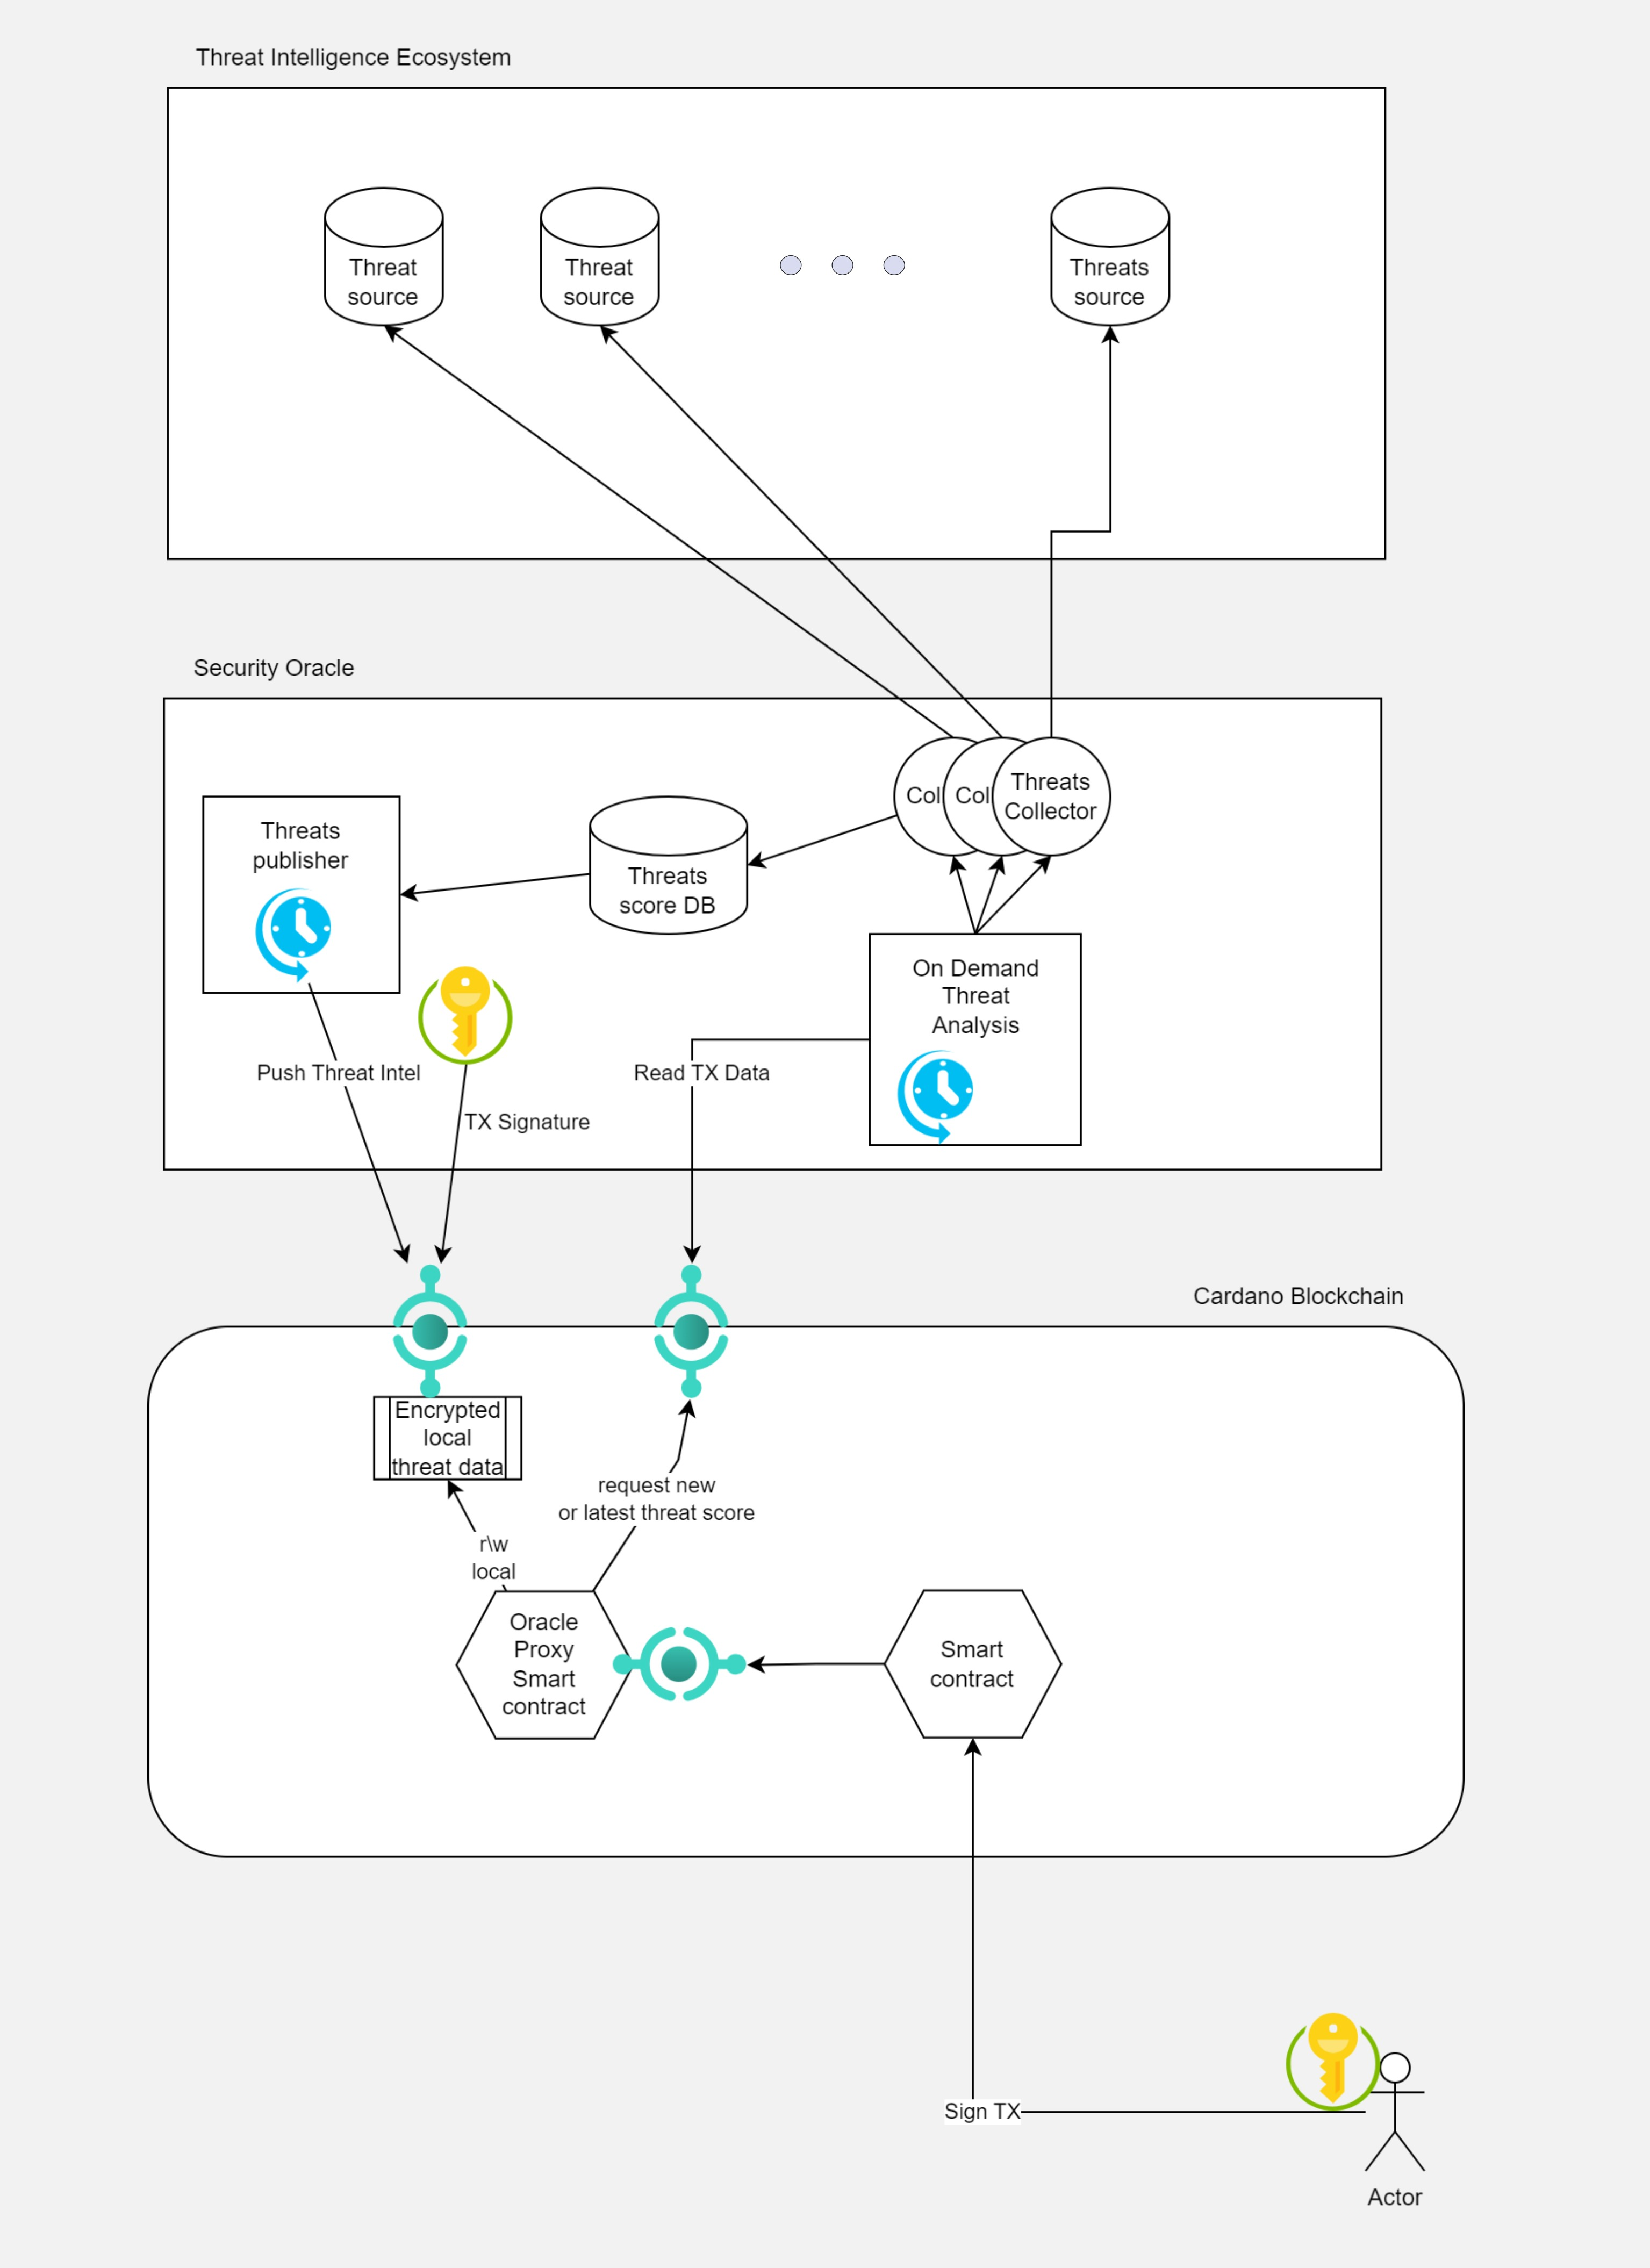
\includegraphics[width=\textwidth]{Images/ComponentsDiagram.jpg}
\caption{Components of the Security Oracle System}
\label{fig:components_diagram}
\end{figure}

% Placeholder for Dataflow Diagram with Simplified Model
\begin{figure}[H]
\centering
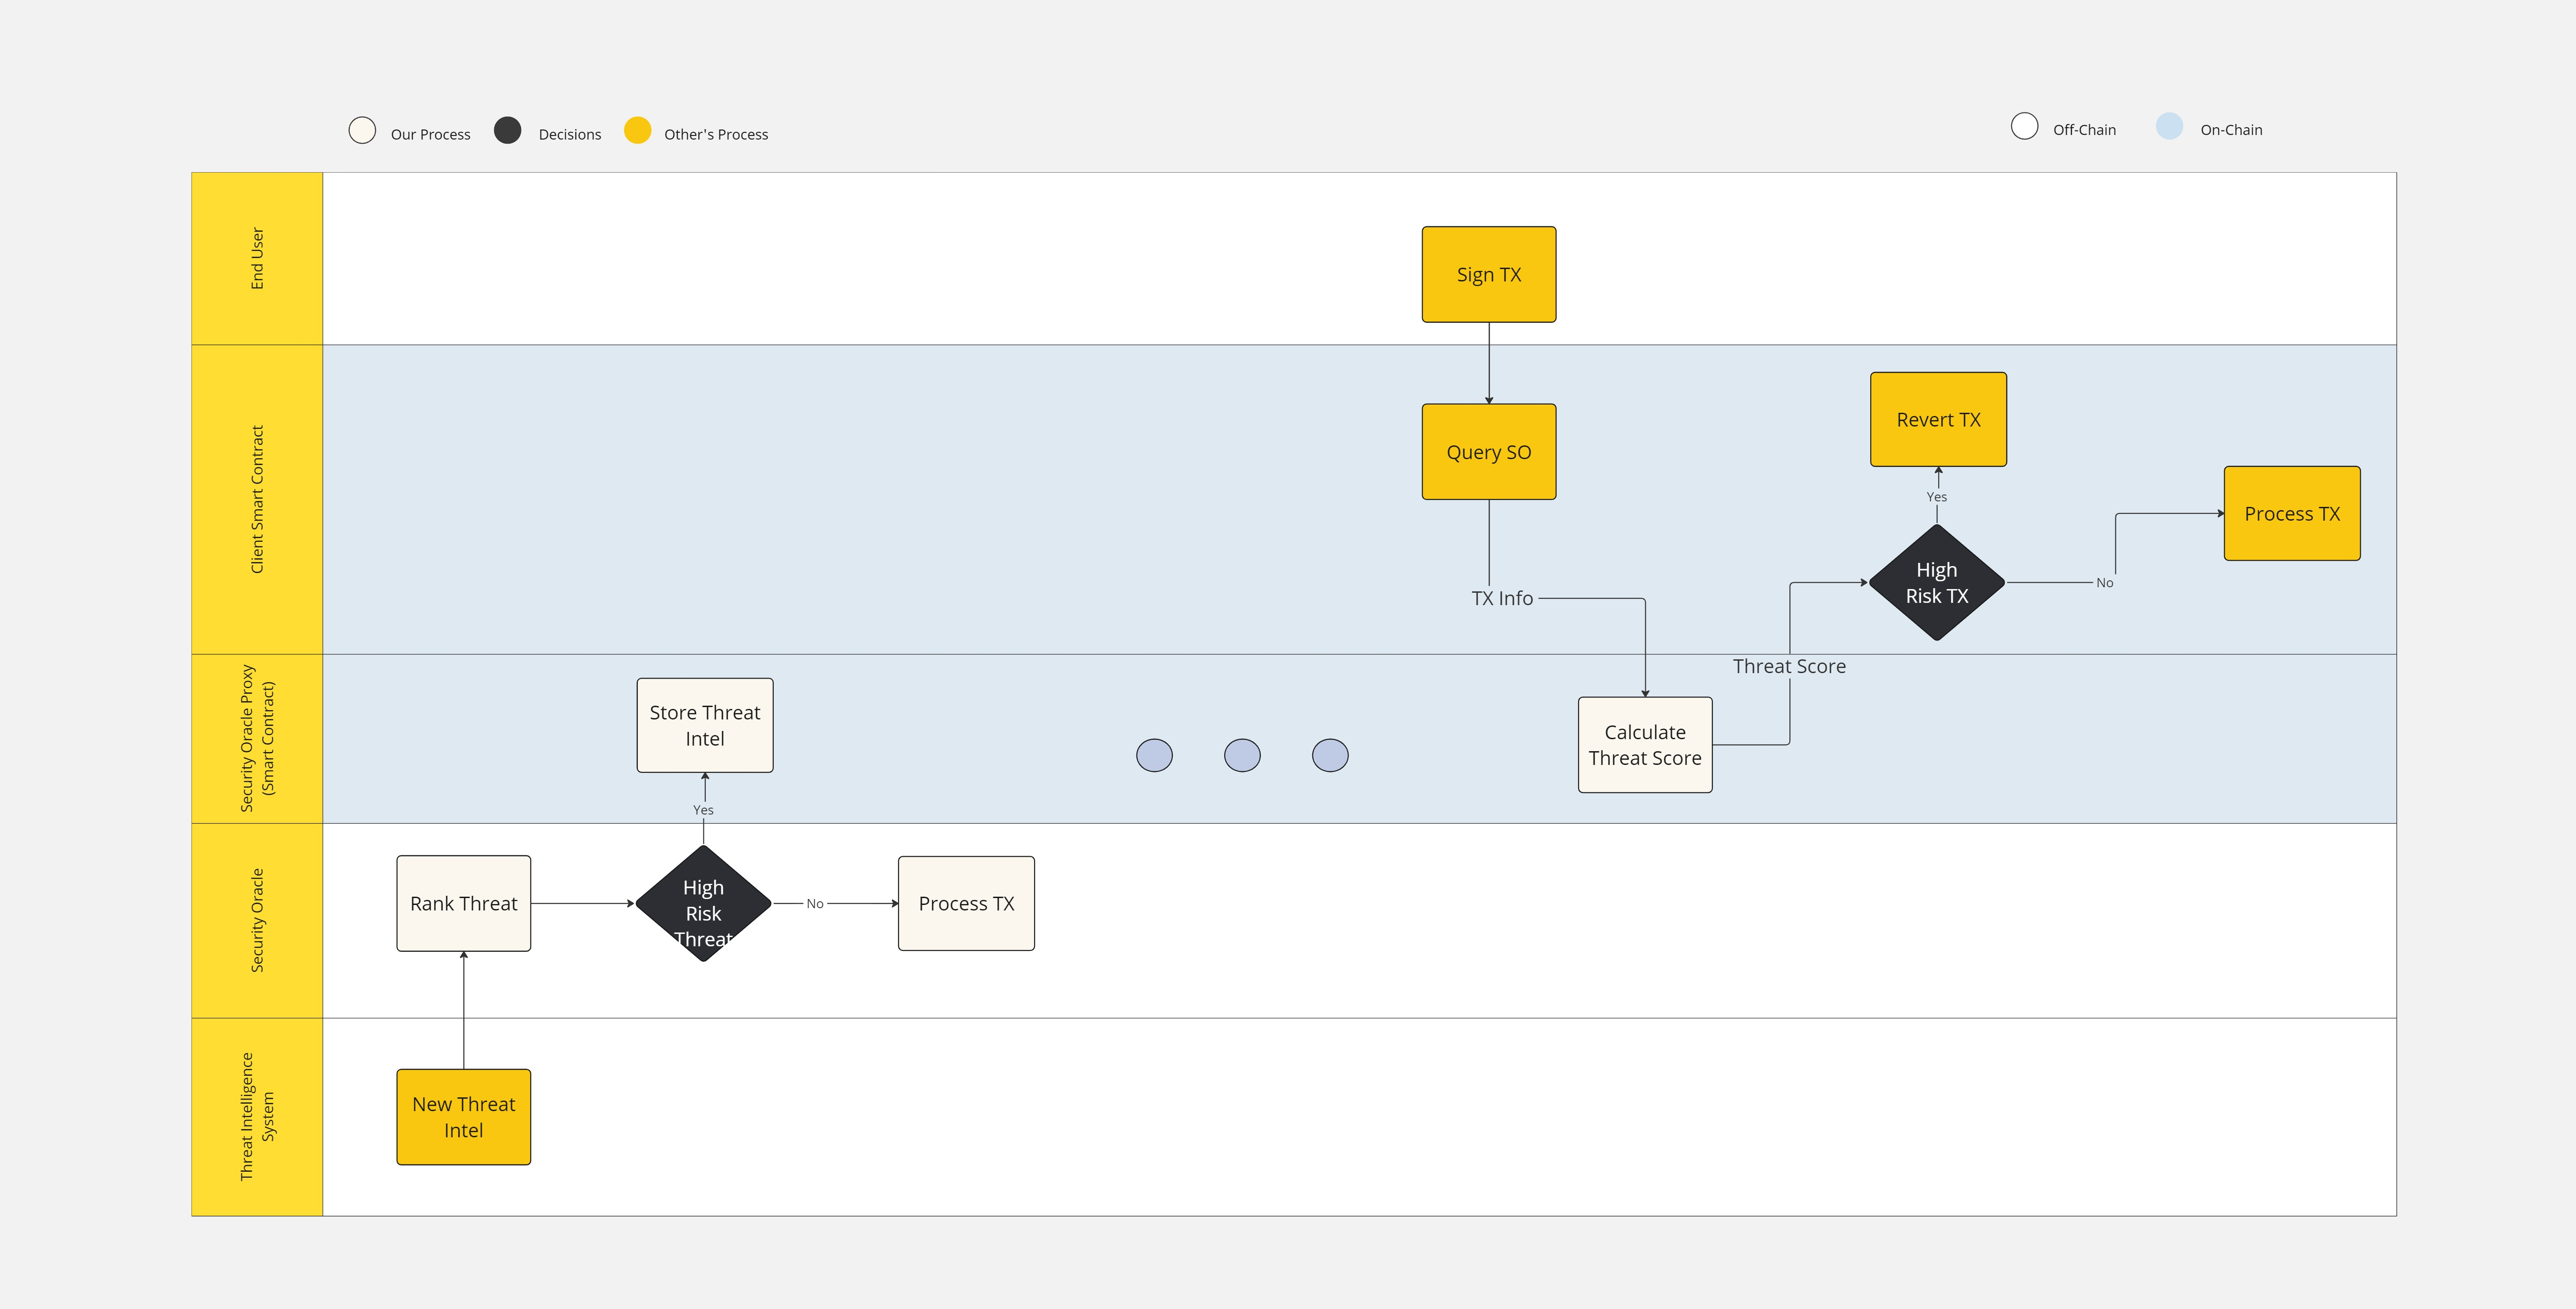
\includegraphics[width=\textwidth]{Images/DataflowDiagramSimple.jpg}
\caption{Dataflow Diagram - Simple Model}
\label{fig:dataflow_simple_diagram}
\end{figure}

% Placeholder for Dataflow Diagram with Pull Model
\begin{figure}[H]
\centering
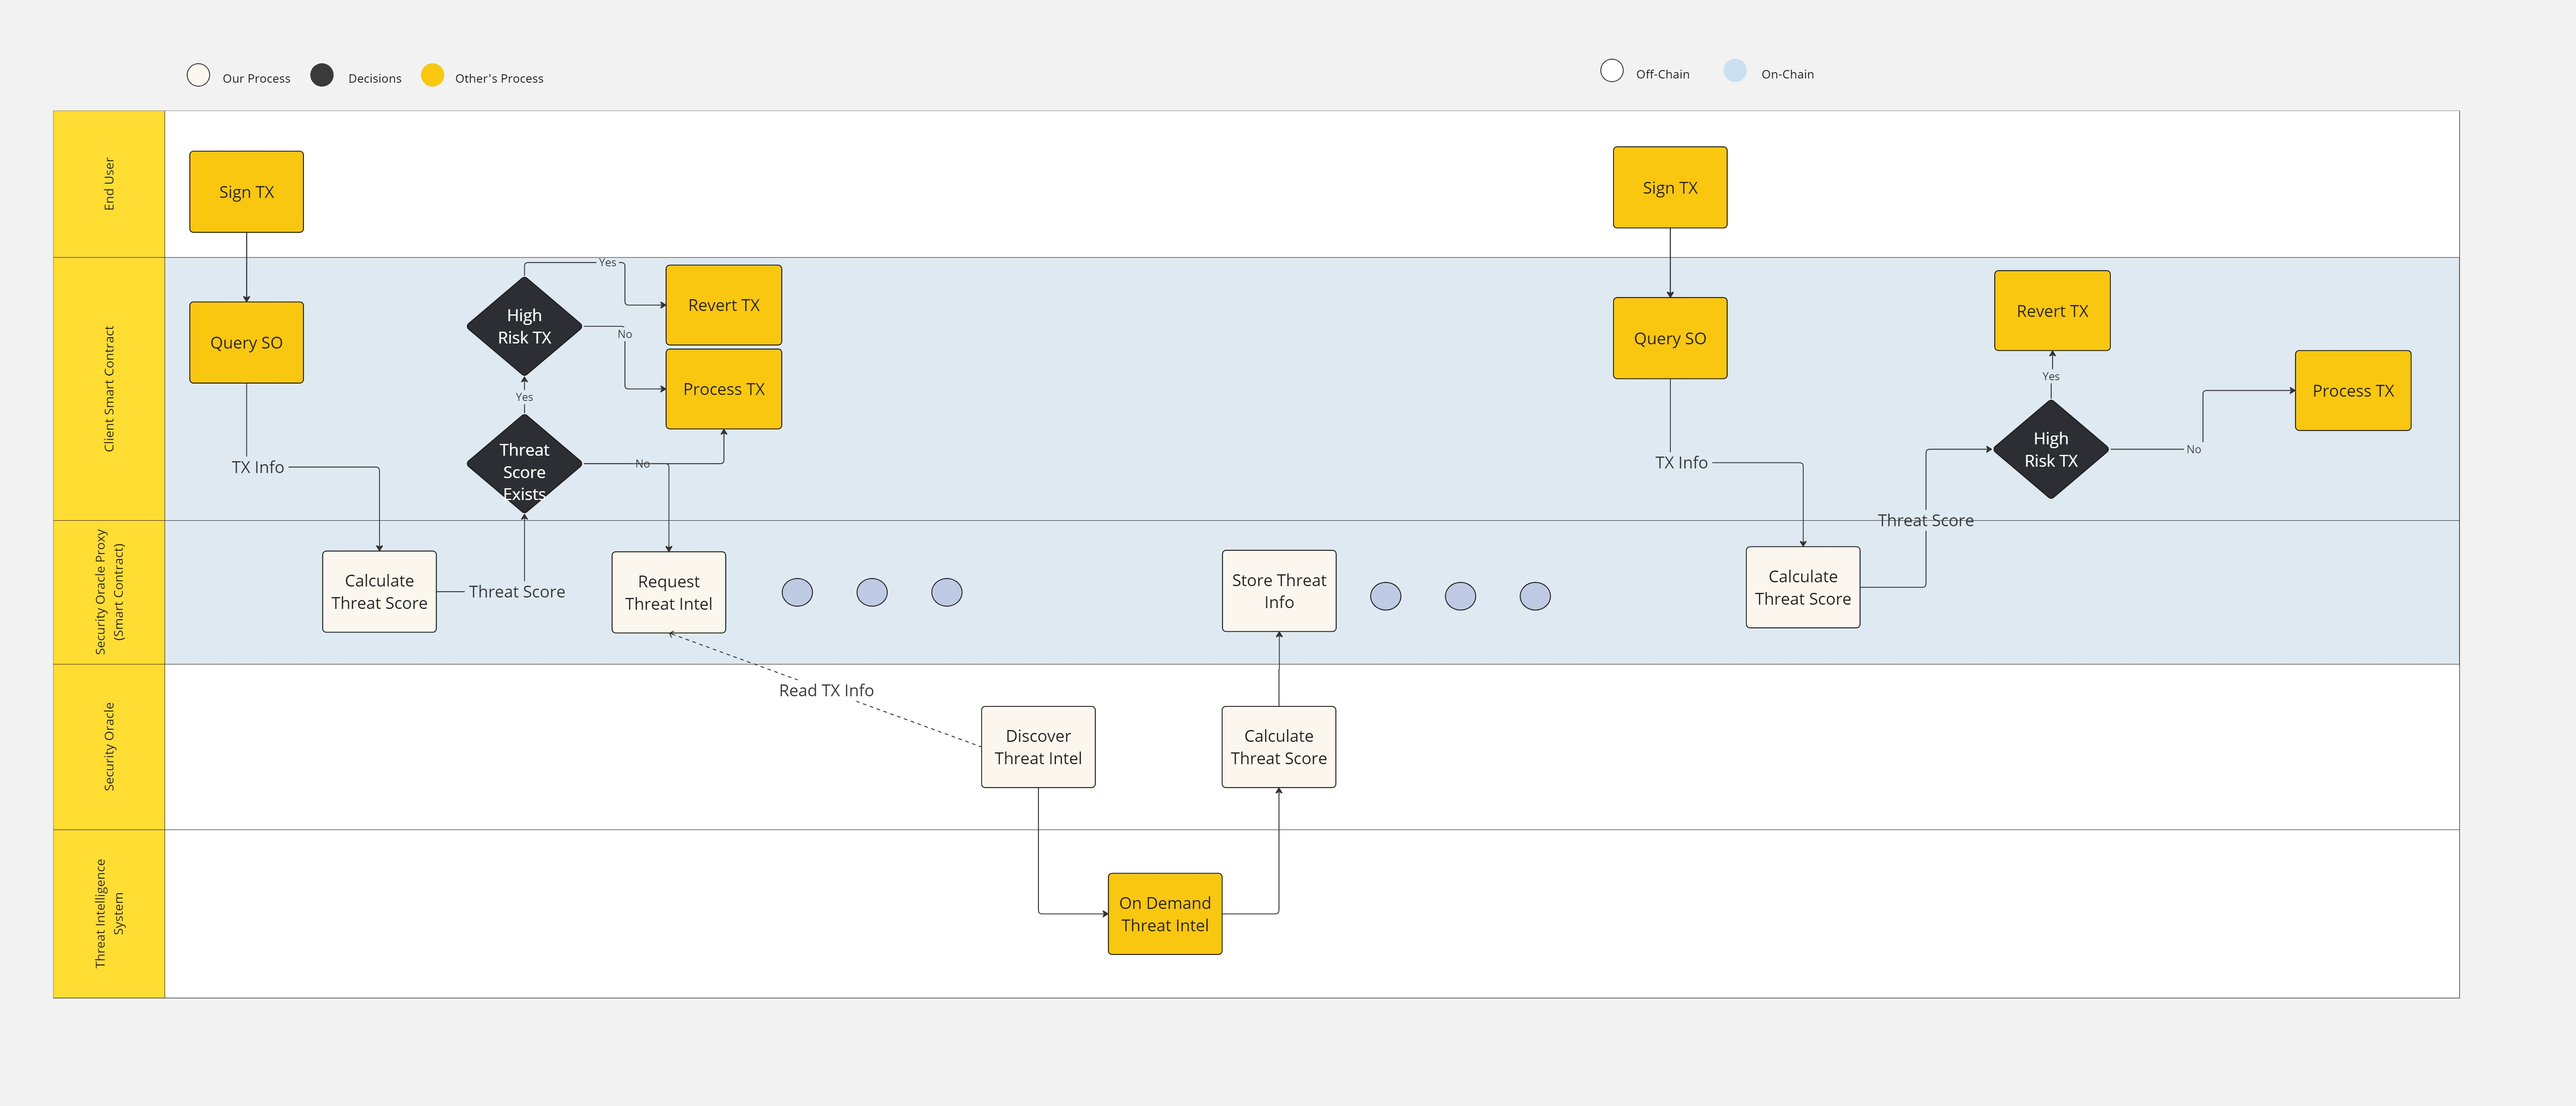
\includegraphics[width=\textwidth]{Images/DataflowDiagramPull.jpg}
\caption{Dataflow Diagram - "On Demand" Threat Analysis}
\label{fig:dataflow_pull_diagram}
\end{figure}


\section{Project Plan}

The project plan for the Security Oracles Proof of Concept (PoC) is delineated through a series of structured milestones, each with specific objectives that guide the development process from inception to completion. Below is a Gantt chart that visually represents the timeline and interdependencies of these milestones.

\begin{figure}[H]
\centering
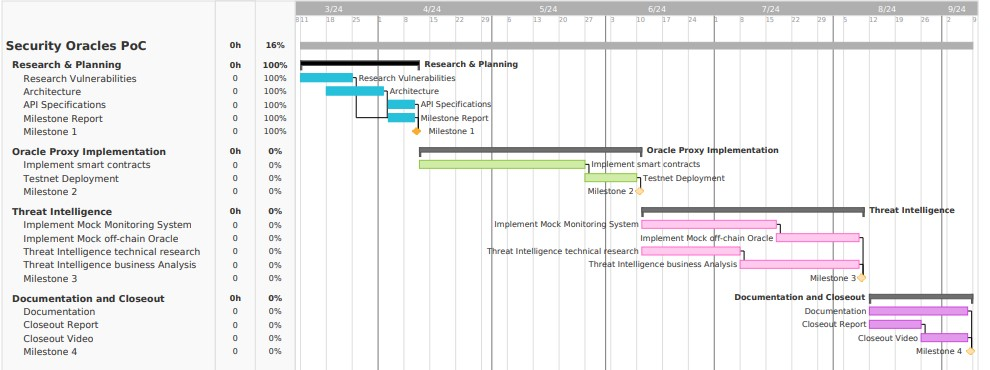
\includegraphics[width=\linewidth]{Images/Security Oracles - Project Plan.jpg}
\caption{Gantt Chart for the Security Oracles PoC Project Plan}
\label{fig:gantt_chart}
\end{figure}

The Gantt chart illustrates the project's progression over a 25-week period, broken down as follows:

\begin{itemize}
  \item \textbf{Milestone 1 (Weeks 1-4):} Research and Planning, including the exploration of vulnerabilities and architectural design, culminating in the Milestone Report.
  \item \textbf{Milestone 2 (Weeks 5-12):} Oracle Proxy Implementation, where smart contracts are developed and deployed to the testnet.
  \item \textbf{Milestone 3 (Weeks 13-20):} Threat Intelligence Monitoring System is developed, with technical research and business analysis taking place to inform its implementation.
  \item \textbf{Final Milestone (Weeks 21-25):} Documentation and Closeout, where all documentation is finalized and a closeout report and video are produced.
\end{itemize}

The planned milestones are crafted to ensure that each phase of the project builds upon the last, with time allocated for the necessary research, development, testing, and documentation required to deliver a comprehensive solution for enhancing smart contract security on the Cardano blockchain.

\appendix
\chapter{References}

Our reseach included discussions with the following organizations - 
\begin{itemize}
    \item \textbf{\href{https://cardanofoundation.org/}{Cardano Foundation}} multiple teams (Finance, partnership, tech support)
    \item \textbf{\href{https://minswap.org/}{Minswap}}
    \item \textbf{\href{https://muesliswap.com/swap}{Muesliswap}}
    \item \textbf{\href{https://github.com/input-output-hk/Certification-working-group}{Certification Working Group}}
    \item \textbf{\href{https://www.geniusyield.co/}{Genius Yield}}
    \item \textbf{\href{https://gimbalabs.com}{Gimbalabs}}
    \item \textbf{\href{http://Sidan.io}{SIDAN}}
    \item \textbf{\href{https://emurgo.io/}{Emurgo}}
\end{itemize}


The following audit reports were included in the analysis - 
\begin{itemize}
    \item \href{https://vyfi-docs.s3.amazonaws.com/initial-audit-report.pdf}{VyFi DEX Initial Audit Report v3 (vyfi-docs.s3.amazonaws.com)}
    \item \href{https://indigoprotocol1.medium.com/indigo-protocol-tweag-security-audit-report-949b3c359f17}{Indigo Protocol: Tweag Security Audit Report | by Indigo | Medium}
    \item \href{https://skynet.certik.com/projects/wingriders}{WingRiders - CertiK Skynet Project Insight}
    \item \href{https://skynet.certik.com/projects/minswap}{Minswap - CertiK Skynet Project Insight}
    \item \href{https://cdn.sundaeswap.finance/audits/mehen.pdf}{Mehen - Fiat-backed Stablecoin (sundaeswap.finance)}
    \item \href{https://github.com/runtimeverification/publications/blob/main/reports/smart-contracts/SundaeSwap.pdf}{publications/reports/smart-contracts/SundaeSwap.pdf at main · runtimeverification/publications · GitHub}
\end{itemize}

The following articles contributed to our research - 
\begin{itemize}
    \item \href{https://minswap-labs.medium.com/vulnerability-patch-technical-details-and-steps-forward-97f6ee35aa91}{Vulnerability Patch: Technical Details and Steps Forward | by Minswap Labs}
    \item \href{https://www.wafflecapital.xyz/blog/zero-hacks}{Zero Hacks - Waffle Capital}
    \item \href{https://m.youtube.com/watch?v=RnshfdRwTSI}{Daedalus Turbo \& Security (Charles Hoskinson, March 15th 2024)}
    \item \href{https://forum.cardano.org/t/smart-contracts-and-their-challenges/54870}{Smart contracts and their challenges - Cardano Forum}
    \item \href{https://plutonomicon.github.io/plutonomicon/vulnerabilities}{Common Plutus Vulnerabilities – Plutonomicon}
    \item \href{https://github.com/IntersectMBO/cardano-ledger/issues/3965}{Reference scripts for `PlutusV1` · Issue \#3965 · IntersectMBO/cardano-ledger · GitHub}
\end{itemize}


\end{document}
